\section{Spotifyとの連携 \index{spotify@Spotify}}
\label{sec:spotify1}
    \subsection{Spotify側の設定}
    \label{sec:spotify2}
        \subsubsection{Spotify for Developersの認証 \index{spotifyfordevelopers@Spotify for Developers}}
        \label{sec:spotify3}
            \begin{enumerate}
                \item \href{https://developer.spotify.com}{Spotify for Developers}にアクセスし、ご利用のSpotifyアカウントでログインしてください。
                \label{item:spotify1}
                \item アカウント名を押下してメニューを表示し、\ttbox{Dashboard}を押下して\spotifydashboard へ移動してください。
                \label{item:spotify2}
                    \begin{figure}[htbp]
                        \centering
                        \fbox{
                            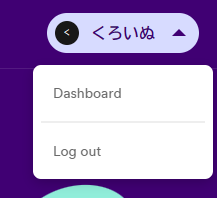
\includegraphics[width=5cm]{./pictures/spotify1.png}
                        }
                        \caption{メニューのDashboard}
                        \label{img:spotify1}
                    \end{figure}

                \item \spotifydashboard で
                    \begin{screen}
                        \texttt{You need to verify your email address (アカウントに登録されているメールアドレス) before you can create an app.}
                    \end{screen}
                    と表示されている部分の\ttbox{Update email address}を押下してください。
                \label{item:spotify3}
                    \begin{figure}[htbp]
                        \centering
                        \fbox{
                            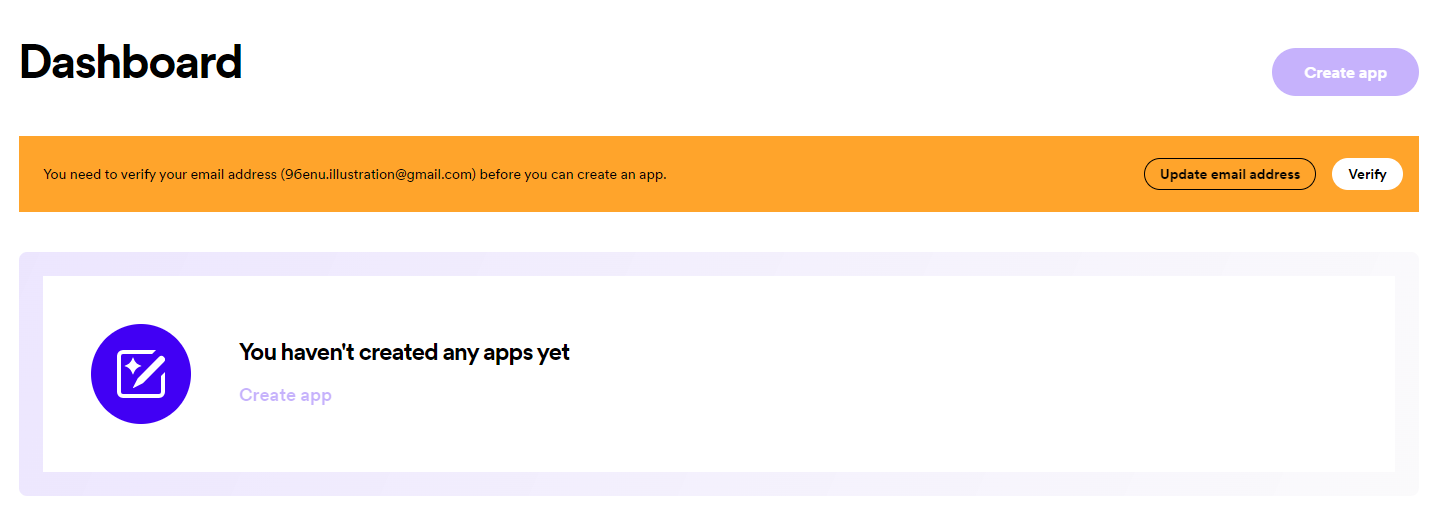
\includegraphics[width=\linewidth]{./pictures/spotify2.png}
                        }
                        \caption{DashboardのUpdate email address}
                        \label{img:spotify2}
                    \end{figure}

                \newpage
                \item \bracketref{item:spotify3}の実行後、アカウントに登録されているメールアドレスに\texttt{no-reply@spotify.com}から\imageref{img:spotify3}のようなセキュリティ確認のメールが送られてくるので、\ttbox{メールアドレスを確認する}を押下してください。
                \label{item:spotify4}
                    \begin{figure}[htbp]
                        \centering
                        \fbox{
                            \includegraphics[width=6cm]{./pictures/Spotify3.png}
                        }
                        \caption{セキュリティ確認のメール}
                        \label{img:spotify3}
                    \end{figure}

                \newpage
                \item ブラウザ上で\imageref{img:spotify4}のようなページが表示されたら、\spotifydashboard に戻ってください。
                \label{item:spotify5}
                    \begin{figure}[htbp]
                        \centering
                        \fbox{
                            \includegraphics[width=6cm]{./pictures/Spotify4.png}
                        }
                            \caption{認証完了画面}
                        \label{img:spotify4}
                    \end{figure}
                \item \spotifydashboard で、\bracketref{item:spotify3}時点では押下できなかった\ttbox{Create app}が押下できるようになっていれば、認証完了です。
            \end{enumerate}

        \newpage
        \subsubsection{Spotifyと\bj 接続用appの作成}
        \label{sec:spotify4}
            \begin{enumerate}
                \item \spotifydashboard の\ttbox{Create app}を押下してください。
                \label{item:spotify6}
                    \begin{figure}[htbp]
                        \centering
                        \fbox{
                            \includegraphics[width=\linewidth]{./pictures/Spotify5.png}
                        }
                        \caption{\spotifydashboard のCreate app}
                        \label{img:spotify5}
                    \end{figure}

                \newpage
                \item \imageref{img:spotify6}のようなapp作成ページが表示されるので、以下を参考に値を設定してください。
                \label{item:spotify7}
                    \begin{figure}[htbp]
                        \centering
                        \fbox{
                            \includegraphics[width=\linewidth]{./pictures/Spotify6.png}
                        }
                        \caption{app作成ページ}
                        \label{img:spotify6}
                    \end{figure}
                    \begin{itemize}
                        \item[\texttt{App name}] なんらかの値を設定してください\footnote{自由な値で構いませんが、\bj 用のappであることが分かるような名前の設定を推奨します。}。
                        \item[\texttt{App description}] なんらかの値を設定してください。
                        \item[\texttt{Website}] 空欄で構いません。
                        \item[\texttt{Redirect URIs}] 必ず\texttt{http://localhost}という値を設定してください。
                        \item[\texttt{Bundle IDs}] 空欄で構いません。
                        \item[\texttt{Android packages}] 空欄で構いません。
                        \item[\texttt{APIs used}] 以下にチェックを入れてください。
                            \begin{itemize}
                                \item \texttt{Android}
                                \item \texttt{Web API}
                            \end{itemize}
                    \end{itemize}

                \newpage
                \item \bracketref{item:spotify7}の項目設定が完了したら、
                \label{item:spotify8}
                    \begin{screen}
                        \texttt{I understand and agree with Spotify's Developer Terms of Service and Design Guidelines}
                    \end{screen}
                    にチェックを入れ、\ttbox{save}を押下してください。

                \item \imageref{img:spotify7}のようなapp Homeページが表示されたら、作成完了です。
                \label{item:spotify9}
                    \begin{figure}[htbp]
                        \centering
                        \fbox{
                            \includegraphics[width=\linewidth]{./pictures/Spotify7.png}
                        }
                        \caption{app Homeページ}
                        \label{img:spotify7}
                    \end{figure}
            \end{enumerate}

        \newpage
        \subsubsection{接続に必要な情報の取得}
        \label{sec:spotify5}
            \begin{enumerate}
                \item \ref{sec:spotify4}で作成したappのHomeページにアクセスし、\ttbox{Settings}を押下してBasic Informationページに移動してください。
                \label{item:spotify10}

                \item ページ上部の\clientId が表示されている枠の\texttt{View client secret}を押下して、\clientSecret を表示してください。
                \label{item:spotify11}
                    \begin{figure}[htbp]
                        \centering
                        \fbox{
                            \includegraphics[width=\linewidth]{./pictures/Spotify8.png}
                        }
                        \caption{Basic Informationページ上部(Client secretを表示する前)}
                        \label{img:spotify8}
                    \end{figure}
                    \begin{figure}[htbp]
                        \centering
                        \fbox{
                            \includegraphics[width=\linewidth]{./pictures/Spotify9.png}
                        }
                        \caption{Basic Informationページ上部(\clientSecret を表示した後)}
                        \label{img:spotify9}
                    \end{figure}

                \item 以下の項目を控えてください。
                \label{item:spotify12}
                    \begin{itemize}
                        \item \clientId
                        \item \clientSecret
                    \end{itemize}
            \end{enumerate}

            \begin{itembox}[c]{\ttbox{!注意!}}
                \texttt\clientId ,\clientSecret は他人に知られないように管理してください。アカウントへの不正アクセス・乗っ取り等が発生する危険があります。
            \end{itembox}

    \newpage
    \subsection{\bj 側の設定}
    \label{sec:spotify6}
        \begin{enumerate}
            \item 設定画面の\ttbox{Spotify接続設定(プレビュー版)}を押下して、設定項目を展開してください。
                \begin{figure}[htbp]
                    \begin{minipage}[b]{0.45\linewidth}
                        \centering
                        \fbox{
                            \includegraphics[width=5cm]{./pictures/Spotify10.png}
                        }
                        \caption{展開前}
                        \label{img:spotify10}
                    \end{minipage}
                    \begin{minipage}[b]{0.45\linewidth}
                        \centering
                        \fbox{
                            \includegraphics[width=5cm]{./pictures/Spotify11.png}
                        }
                        \caption{展開後}
                        \label{img:spotify11}
                    \end{minipage}
                    \caption*{Spotify接続設定(\currentVersion)}
                \end{figure}

            \newpage
            \item \ref{sec:spotify5} \bracketref{item:spotify12}で控えた\clientId ,\clientSecret を\ttbox{Spotify接続設定(プレビュー版)}に入力してください。
                \begin{figure}[htbp]
                    \centering
                    \fbox{
                        \includegraphics[width=5cm]{./pictures/Spotify12.png}
                    }
                    \caption{\clientId ,\clientSecret を入力}
                    \label{img:spotify12}
                \end{figure}

            \newpage
            \item \ttbox{Spotify接続設定(プレビュー版)}の\ttbox{接続テスト}ボタンが押下できるようになるので、押下して認証ページへアクセスしてください。
            \item \imageref{img:spotify13}のような認証ページが表示されるので、\ttbox{同意する}を押下してください。
                \begin{figure}[htbp]
                    \centering
                    \fbox{
                        \includegraphics[width=5cm]{./pictures/Spotify13.png}
                    }
                    \caption{認証ページ}
                    \label{img:spotify13}
                \end{figure}

            \newpage
            \item 認証ページが閉じ、\imageref{img:spotify14}のような成功ダイアログが表示されたらSpotify側の準備は完了です\footnote{ダイアログ内のユーザー名がご自身のアカウントと一致していることを確認してください}。
                \begin{figure}[htbp]
                    \centering
                    \fbox{
                        \includegraphics[width=5cm]{./pictures/Spotify14.png}
                    }
                    \caption{認証ページ}
                    \label{img:spotify14}
                \end{figure}
        \end{enumerate}

    \newpage
    \subsection{Spotify連携時の挙動について}
    \label{sec:spotify7}
    \begin{itemize}
        \item 約1分に一度、Spotifyで再生中の曲を確認し\mi への\nowplaying を行います。
        \item 以下のいずれかに該当する場合、\nowplaying を行いません。
        \begin{itemize}
            \item 再生中の曲がない
            \item \mi の\accessToken が設定されていない
            \item \nowplaying が有効になっていない
            \item 前回の\nowplaying と曲名・アーティスト名が変化していない
            \item スマートフォンがネットワークに接続されていない
            \item スマートフォンがロック状態になっている\footnote{ディスプレイを常時表示設定にすることで、解決する場合があります}
        \end{itemize}
    \end{itemize}
